\subsection{Results}


\begin{figure}[H]
\centering
\makebox[\textwidth][c]{
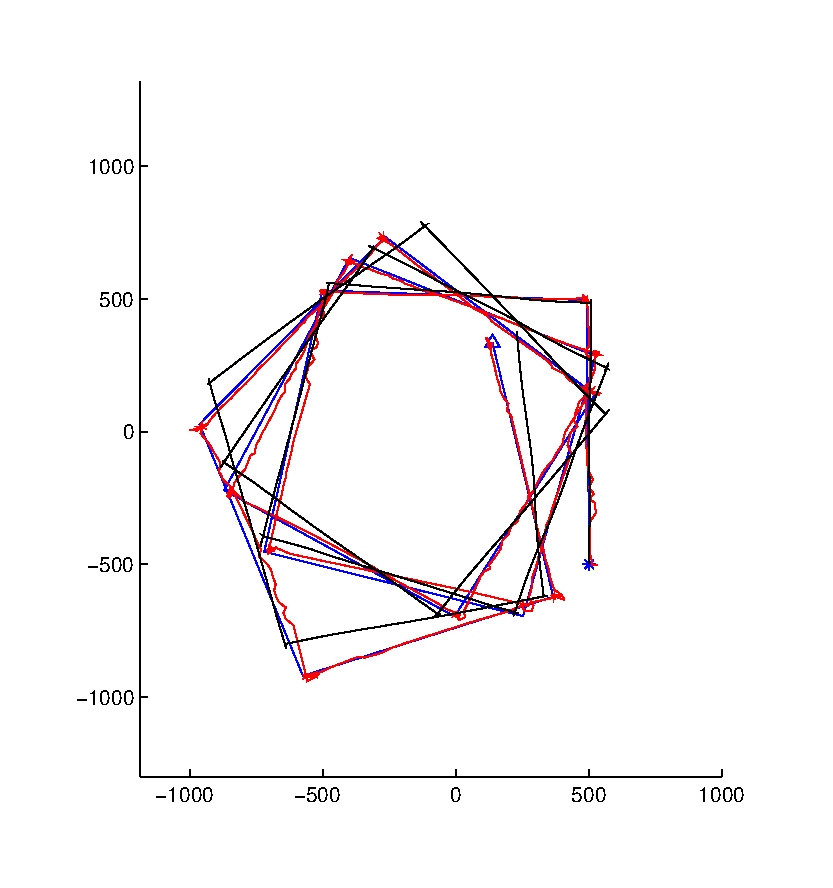
\includegraphics[width = 15cm,trim= 1cm 1cm 1cm 1cm ,clip=true]{graphics/comparison_encoderVSscanner}}
\caption[Comparison of the two localization methods.]{Comparison of the two localization methods. The blue line is the actual path travelled, $*$ is start and $\Delta$ is end. The Red line is the 2D Laser Scanner and the black line the encoder data.}
\label{fig:comparisonOfEncoderVSScanner}
\end{figure}